\documentclass[preprint]{sigplanconf}

% The following \documentclass options may be useful:
%
% 10pt          To set in 10-point type instead of 9-point.
% 11pt          To set in 11-point type instead of 9-point.
% authoryear    To obtain author/year citation style instead of numeric.

%% wget http://drupal.sigplan.org/sites/default/files/sigplanconf.cls

%% To compile under Ubuntu:
%% cd Calico/papers/dsl-13/
%% sudo apt-get install texlive-latex-base
%% sudo apt-get install texlive-fonts-recommended
%% make

\usepackage{amsmath}
\usepackage{graphicx}

\begin{document}

\conferenceinfo{SPLASH DLS'13}{October 28, 2013, Indianapolis, Indiana, USA.} 
\copyrightyear{2013} 
\copyrightdata{ACM} 

\titlebanner{Submitted to SPLASH DLS'13; Under review}        % These are ignored unless
%%\preprintfooter{short description of paper}   % 'preprint' option specified.

\title{Calico: An Ecosystem for Dynamic Languages}
%% \subtitle{Subtitle Text, if any}

\authorinfo{Douglas S. Blank}
           {Bryn Mawr College\\Department of Computer Science\\Bryn Mawr, PA 19010}
           {dblank@cs.brynmawr.edu}

\authorinfo{Mark F. Russo}
           {Affiliation2}
           {Email2}

\authorinfo{James B. Marshall}
           {Affiliation3}
           {Email3}

\maketitle

\begin{abstract}
This is the text of the abstract.
\end{abstract}

\category{CR-number}{subcategory}{third-level}

\terms
term1, term2

\keywords
keyword1, keyword2

\section{Overview}

The Calico Project defines a collection of technologies designed to
create an ecosystem for dynamic languages. The Calico ecosystem has a
number of interesting properties: 1) allows multiple dynamic languages
to interact and interoperate; 2) libraries written for the ecosystem
are usable by all of the languages as if they were native to each
language; 3) provides a smooth continuum of experience for the
beginning computer programmer; 4) exposes a unified interface for
exploring a variety of dynamic languages; and 5) is an open-source
testbed for developing new concepts in dynamic languages. As such,
Calico defines a useful ecosystem for students, educators, and
developers wishing to explore computer science and pedagogy.

Calico is defined by three layers of technologies: a virtual computer,
a Dynamic Language Runtime (DLR), and support libraries and
executables. In addition, an Integrated Development Environment (IDE)
pulls all of these pieces together. As implemented, Calico languages
can all live and operate in the same space, share variables and code,
and the code can run competitively fast. The following sections go
into the details of each of the pieces that comprise the Calico
ecosystem.

\subsection{Universal Virtual Computer}

At the foundation of Calico is what could be characterised from the
programmer's perspective as a universal virtual computer. The dynamic
language programmer should be able to write code capable of modern
functionality without having to worry about the details of the
operating system or underlying hardware. For example, the programmer
should be able to write programs capable of: turning text to speech;
playing audio files; defining functions that can be used for tone
generation; creating graphical user interfaces with unconstrained
drawing abilities; reading and writing standard image formats; and
providing access to modern input/output hardware devices, such as
gamepads, joysticks, webcams, and robots. In addition, such a system
should be easy to install and maintain, with limited need for
platform-specific dependencies. Finally, we believe that a long term
platform for research and education should be free, both in terms of
price and ability to distribute and alter. This section examine the
components of a universal virtual computer.

\subsubsection{Virtual Machine}

A large portion of the universal virtual computer is defined by a
``process virtual machine.'' There are a number of process virtual
machines (VMs) one could use for a dynamic language ecosystem. We
wanted a VM with a large and active development community, and so
excluded more narrowly-focused VMs such as the Squeak Virtual Machine
(http://www.squeak.org/Features/TheSqueakVM/). Oracle's Java and
Microsoft's .NET are two VMs that both define viable possibilities:
both have object-oriented programming languages, compilers, and
associated virtual machines and runtimes. The Java VM (JVM) has the
Java language (among other possibilities), and .NET has C\# (among
other possibilities). Both systems compile to bytecode that is
executed by their respective virtual machines' runtime.

Although both VMs have served as the foundation for dynamic languages,
Java does not have a complete and robust official open-source
implementation. On the other hand, .NET’s virtual machine components,
called the Common Language Infrastructure (CLI), have been clearly
defined in a pair of Ecma standards, specifically Ecma \#334 and Ecma
\#335 (Ecma Standards, 2011), and is protected by a promise from
Microsoft not to sue (Microsoft Community Promise, 2007). More
importantly, these standards have been implemented independently by
Mono as open source. We have put a high value on having a complete and
open source ``stack'' of robust software layers. Although one could
debate which system is more ``open'', we decided to select the CLI as
implemented by Mono. we will refer to Mono's implementation of the CLI
as MVM (for Mono Virtual Machine).

However, we are not limited to only MVM-based technologies. Using IKVM
(described below) we are able to utilize code compiled for the Java
VM. In this manner, we have assembled components that bring together
the best of both of these two virtual machine systems. In effect, we
have a ``universal virtual machine'' that can use a wide variety of
available open-source libraries on a varied set of operating
systems. One such library is the Dynamic Language Runtime described in
the next section.

\subsubsection{Dynamic Language Runtime}

Although the MVM and the JVM both define everything necessary to
implement a dynamic language, neither has built-in support for
allowing such dynamic languages to interoperate. That is, even though
a variety of languages can be compiled to either VM, there is little
common infrastructure in the VM itself. Without a dynamic language
infrastructure, it is difficult for languages to share environments,
data structures, objects, or functions. Two Java Specification
Requests have been made to add such functionality to Java: JSR-223
would add language hosting and JSR-292 would add dynamic binding (Wu,
2010). There are a number of projects underway to make the JVM more
flexible for use with dynamic languages, including: the Da Vinci
Machine as the reference implementation of JSR-292; Project Lambda
adds lambda to the JVM; Project Jigsaw adds supported for importing
versioned modules; and Nashhorn adds caches for dynamic invokes. When
complete, these technologies will extend the Java technologies to make
them much more suitable for dynamic languages.

The MVM has an existing, mature framework for implementing languages
called the Dynamic Language Runtime (DLR), and at least two dynamic
languages have been written using the DLR: IronPython and
IronRuby. The DLR contains many tools and technologies for language
writers to create languages, and abilities for the languages to
interoperate. Calico includes the DLR, and contains versions of
IronPython and IronRuby.

The DLR contains support necessary for creating, parsing, and
executing modern dynamic languages. [FIXME: add more details about the
  DLR: DynamicObject, cache point, AST, hosting, environment]

\subsection{Supporting Libraries}

To create a universal virtual computer, we need to have a set of
capabilities on top of the virtual machine and dynamic language
runtime that run the gamut from audio to graphics. Of course,
operating systems and hardware vary wildly. Fortunately, there are
open source libraries for the MVM that cover these requirements. For
graphics, we selected Gtk\# which wraps low-level C-based
libraries. For accessing audio and hardware devices (such as
gamepads), we selected the Simple DirectMedia Layer (SDL). SDL is
quite popular in open source, providing additional capabilities for
many projects, including pygame.

[FIXME: Gtk. SDL. espeak. graphviz. ]

The MVM and the above mentioned libraries form the lowest level of the
virtual computer. These libraries are machine-dependent, and those
must be compiled for each platform. We attempted to create the fewest
number of machine-specific dependencies to make the virtual computer
easy to maintain and port to new architectures. The machine-dependent
code is wrapped for consumption by the MVM. Finally, after this
low-level set of dependencies are satisfied, then additional libraries
can be written in a machine-independent fashion using the MVM, or with
the JVM and converted with IKVM.

[FIXME: IKVM]

Combined with the MVM and DLR, these libraries complete the
functionality of a universal virtual computer so that one can write
programs that utilize graphics user interfaces (including widgets,
freestyle pixel manipulation, event handlers, and image formats),
audio (including text-to-speech and tone generation), access to
hardware devices, and other modern functionality. One can then write
in dynamic languages with the full scope of abilities on most of the
operating systems in use, including Windows, Linux, Mac OSX, and
FreeBSD.

\subsection{Integrated Development Environment}

From the user's perspective, an important part of using any
programming language is the user interface. The Calico IDE is designed
to be agnostic to any particular language, or particular use.

\section{Languages}

[FIXME] What defines a Calico language? Document, Engine

First-class languages: stepper, breakpoints, share variables, call
functions, execute/evaluate code and expressions from other languages,
import Calico modules as if they were native.

Second-class: naive ports, minimal interoperation, possibly unable to
import modules.

\subsection{Calico Jigsaw}

Block-based programming languages have facilitated our ability to
introduce computer programming to novice programmers. Perhaps the most
notable example of this is Scratch [http://scratch.mit.edu]. Building
executable programs by plugging together virtual blocks is a concept
that is much less intimidating to [a]beginners, especially when
compared to the precise syntactical rules demanded by many modern
programming languages. For this reason we sought to include a
block-based language as part of the Calico ecosystem. We named our
block language Calico Jigsaw.

The Jigsaw editor provides a palette of blocks that are dragged onto a
canvas using the mouse and connected to form an executable program
Figure~\ref{jigsaw1}. Jigsaw blocks may have properties that can be assigned
values by the programmer. For example, the Jigsaw ``repeat'' block has
a Repetitions property that can be assigned a numeric value indicating
the number of times an inner stack of blocks should be executed. But
beyond the standard functionality expected in any block language,
Jigsaw has several additional features that we feel make it unique.

\begin{figure}[h!]
  \centering
     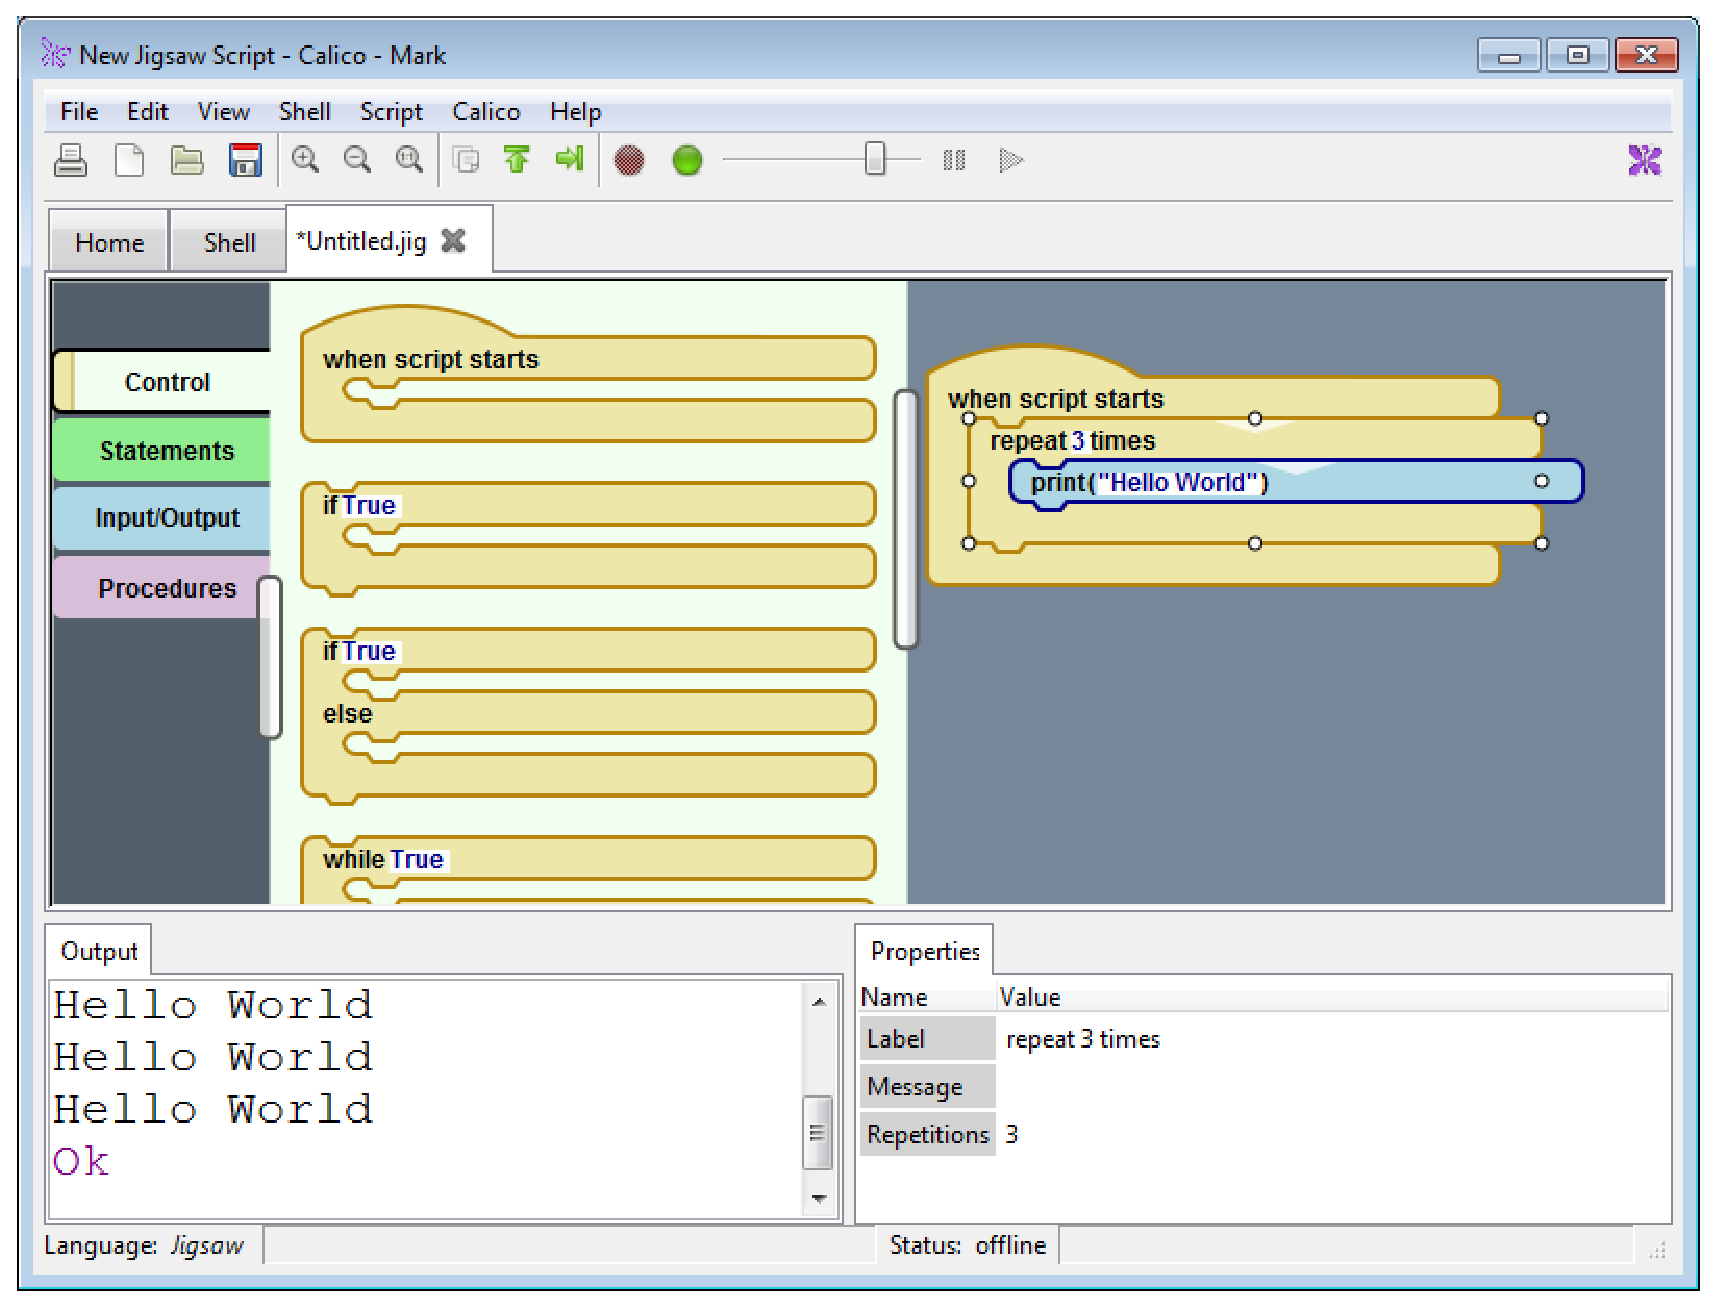
\includegraphics[width=75mm]{jigsaw1.eps}
  \caption{Jigsaw in action.}
  \label{jigsaw1}
\end{figure}

The first important feature worth noting is that Jigsaw is built as a
wrapper around IronPython. Even though Jigsaw is written in C\#, most
Jigsaw statement blocks are implemented as Python statements. This
integration between C\# and IronPython is possible with help from the
DLR. Block statements are compiled and held as compiled code objects
that are ready to be evaluated when the Jigsaw program runs. A
consequence of this design decision is that Python syntax often can be
used directly in Jigsaw. For example, instead of entering primitive
values for block properties, Python expressions can be substituted
instead. The conditional statement in a Jigsaw ``if'' block is a
boolean expression written using Python syntax Figure~\ref{jigsaw2}. We believe
that this approach better prepares the student for a smooth transition
to higher level languages.

\begin{figure}[h!]
  \centering
    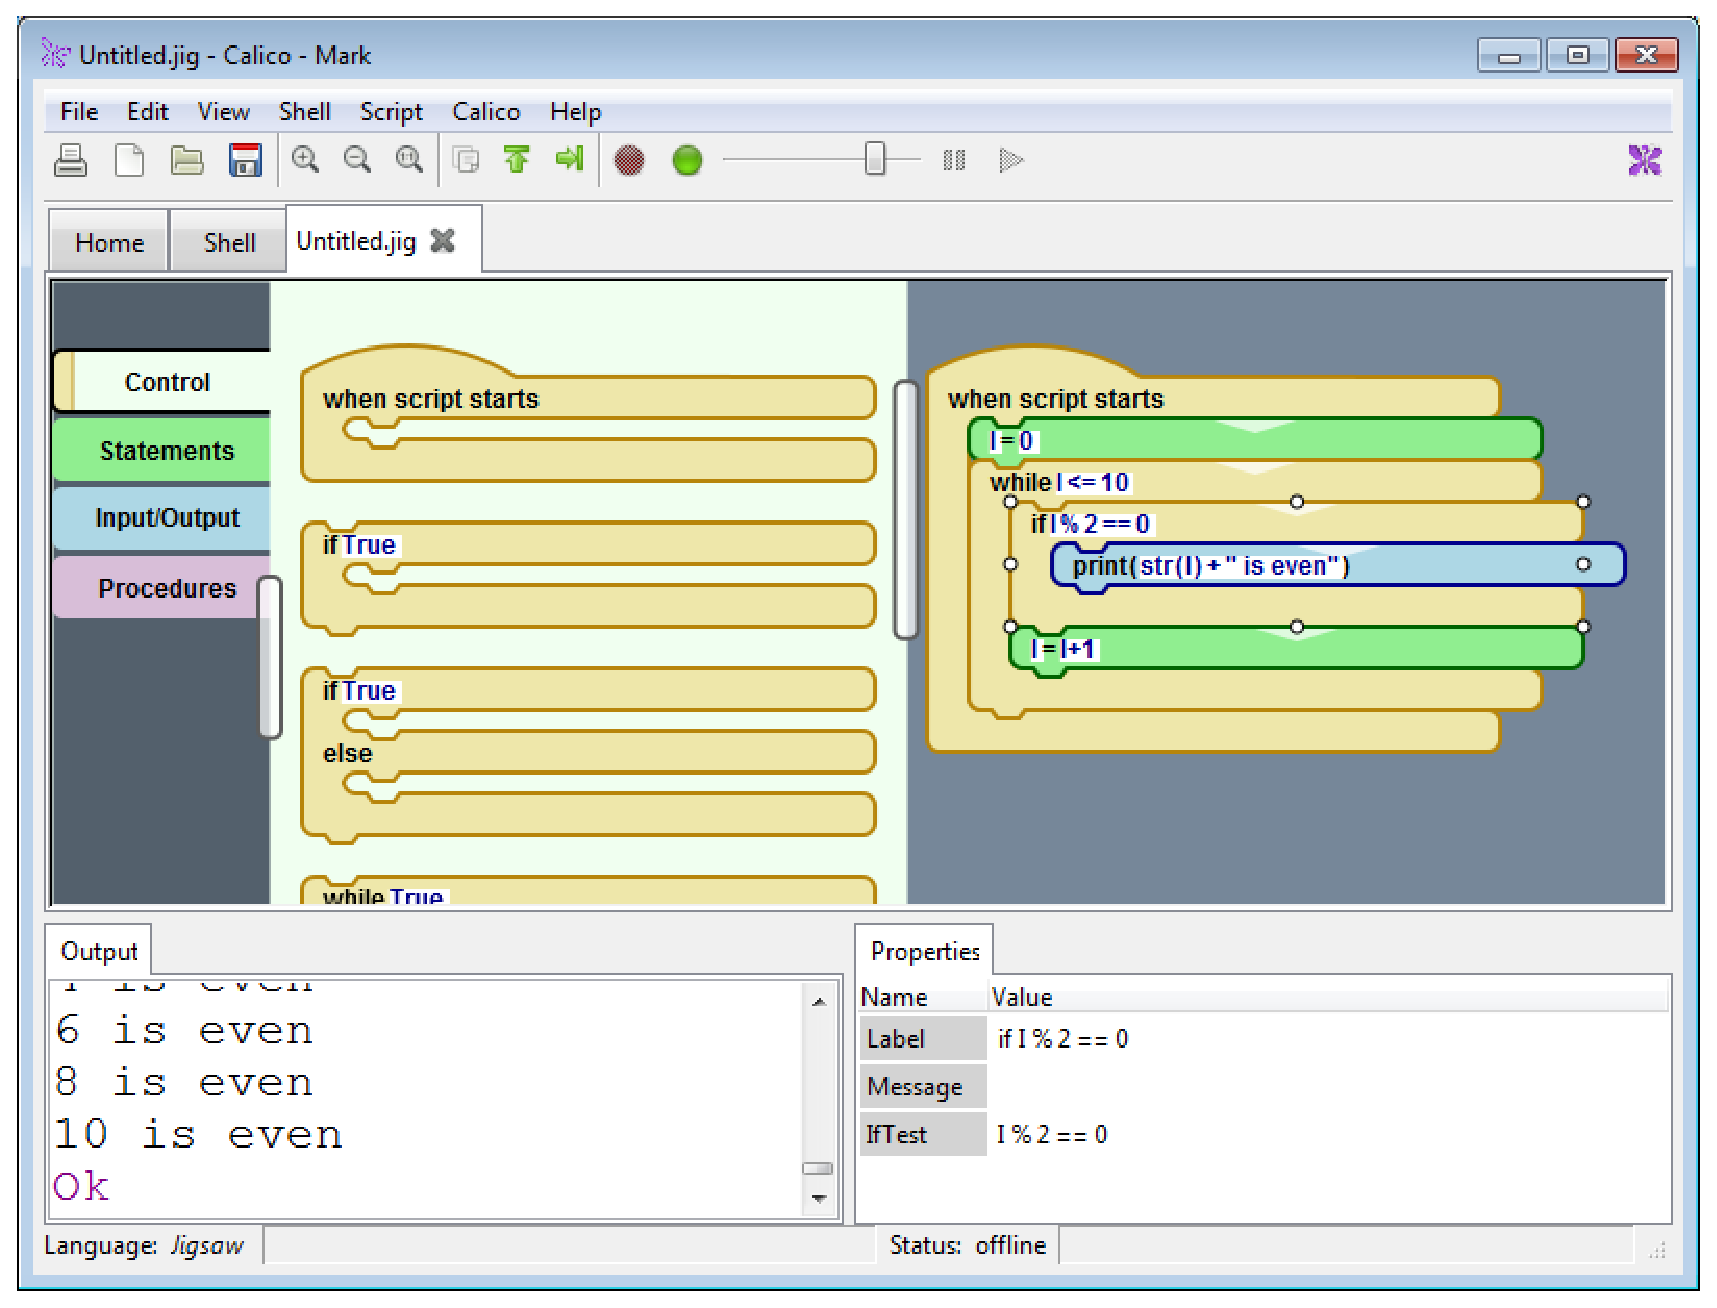
\includegraphics[width=75mm]{jigsaw2.eps} 
  \caption{Jigsaw blocks leverage IronPython expressions.}
  \label{jigsaw2}
\end{figure}

Although many Jigsaw statements and expressions are borrowed from
IronPython, Jigsaw implements it’s own program control
structures. Blocks that provide looping, conditionals and procedures
are all implemented entirely in Mono C\#. Program execution is managed
using Jigsaw’s own implementation of call stacks and stack frames
along with local and global namespaces, an idea that is borrowed from
Python.

Another unique feature of Jigsaw is that it has a form of multitasking
baked in to its execution engine Figure~\ref{jigsaw3}. A Jigsaw program begins
execution at a ``when script starts'' block, and proceeds down the
attached stack of blocks, executing each in sequence. But a Jigsaw
program can contain any number of ``when script starts'' blocks, which
all begin execution at the same time. As a result, multiple block
stacks a Jigsaw program can execute in parallel.

\begin{figure}[h!]
  \centering
    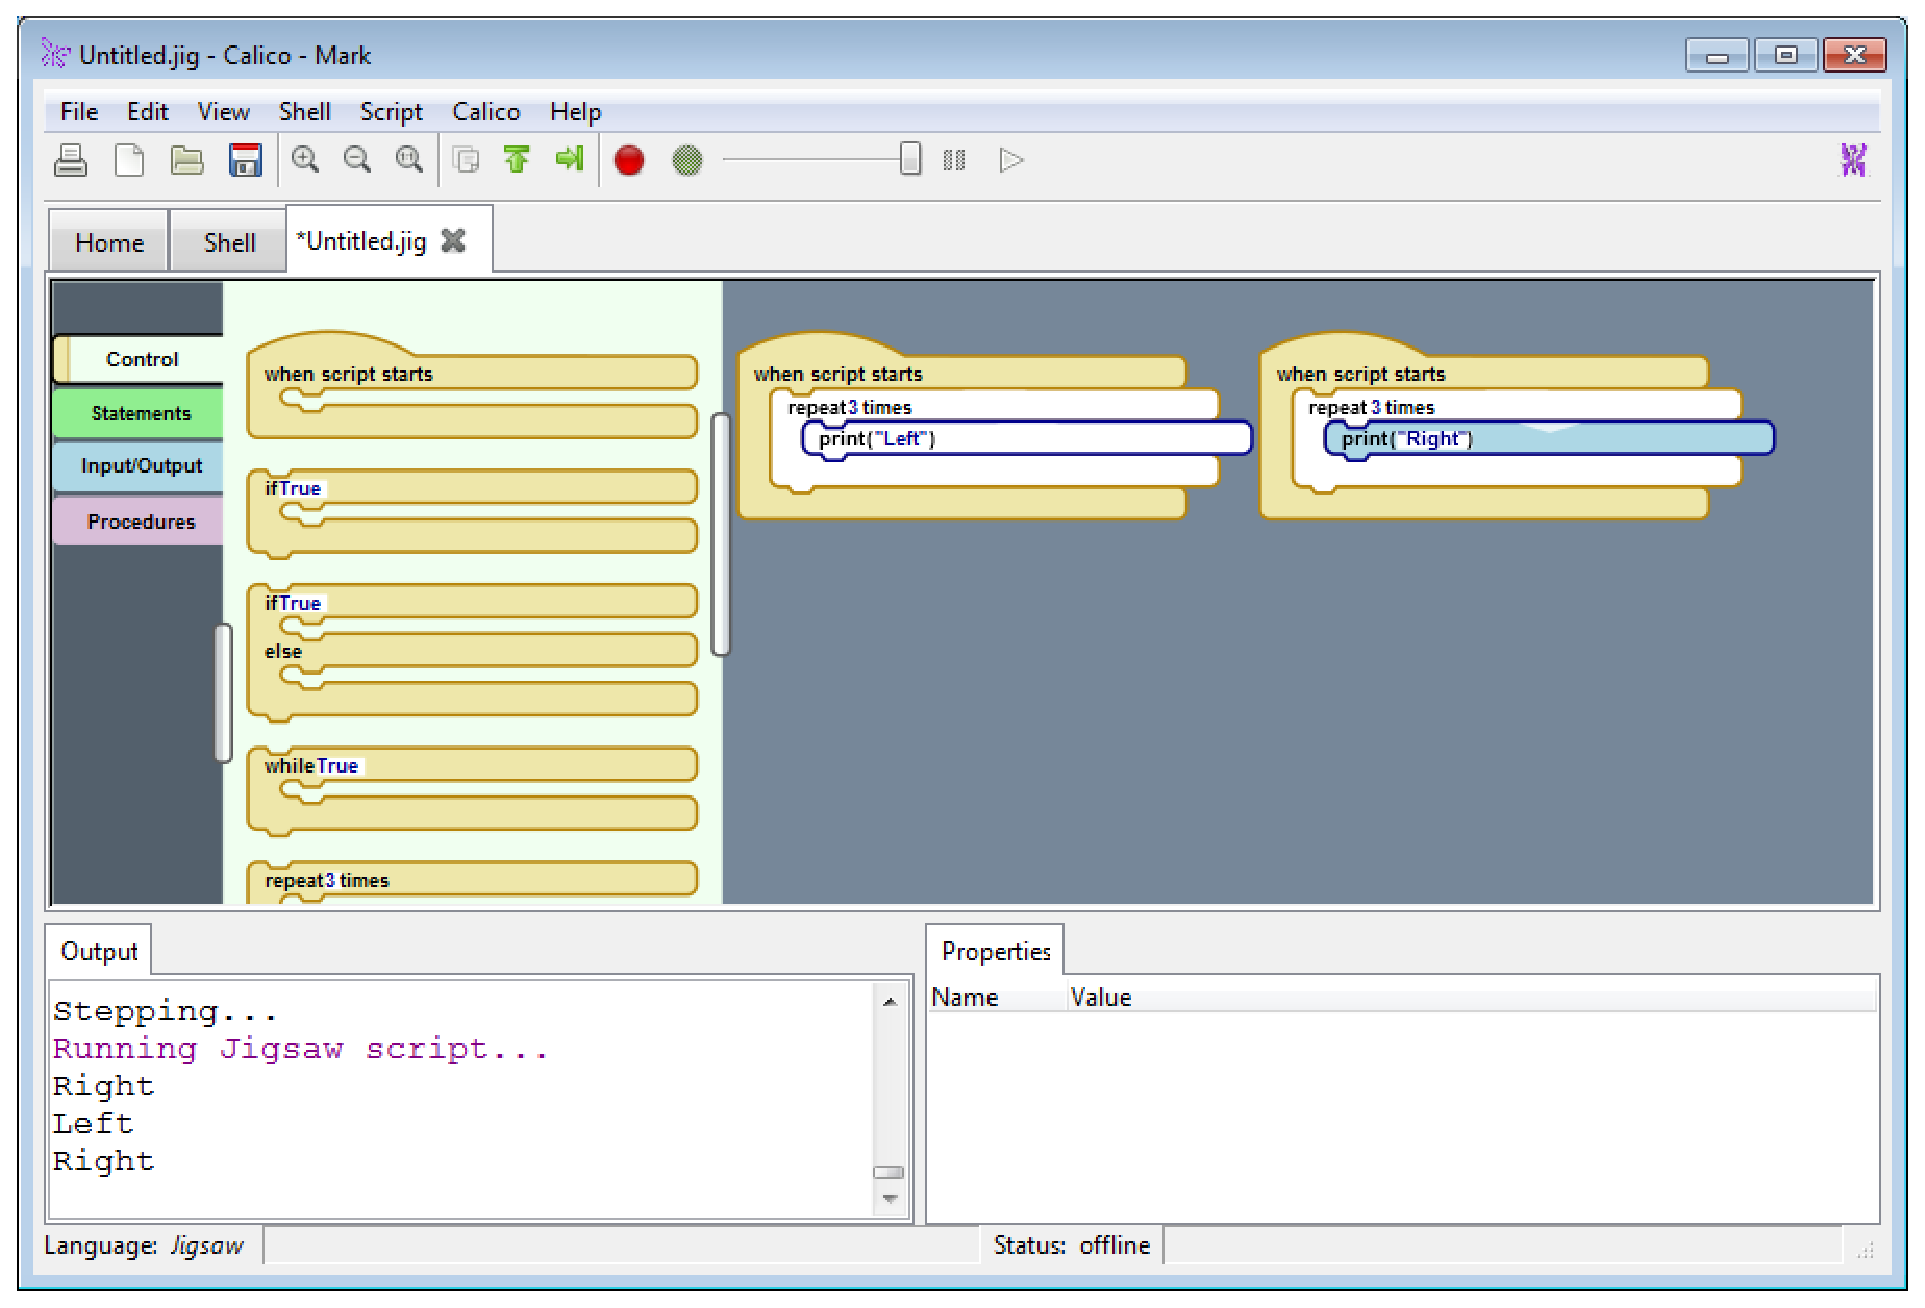
\includegraphics[width=75mm]{jigsaw3.eps} 
  \caption{A Jigsaw programming running multiple block stacks in parallel}
  \label{jigsaw3}
\end{figure}

In fact, the parallelism implemented in Jigsaw is a form of
cooperative multitasking, not the more common preemptive style. Jigsaw
executes multiple block stacks in a round-robin fashion. It is
important to note that the execution of one block does not necessarily
complete before the Jigsaw engine switches to a block in another
stack. Indeed, multiple blocks in different stacks can execute at the
same time. This is possible because the execution element of every
block is implemented as a C\# Enumerator, which is carefully designed
to yield at appropriate times throughout the execution task. With this
style of multitasking a novice programmer can assemble a program
easily that, say, draws graphics to the screen while monitoring a
sensor in the ``background.'' This style of multitasking avoids the
potential for subtle bugs that often crop up with a true preemptive
model.

Calico Jigsaw allows the export of any Jigsaw script to Calico Python
(described below). However, as it must convert Jigsaw's controls to
those of the Python language, the semantics must also be
converted. Figure~\ref{jigsaw4} shows the above Jigsaw program as it
appears after it has been exported to Python. Python does not have the
built-in ability to run functions simultaneously as does Jigsaw. But,
the Calico Myro module (described below) includes a friendly interface
to using threads through the ``doTogether'' function, and so the
export translates the Jigsaw program to the proper form. Notice,
however, that the Output tab indicates that Python's threads do not
guarantee even multitasking as the 'Left' and 'Right' outputs are not
perfectly interleaved.

\begin{figure}[h!]
  \centering
    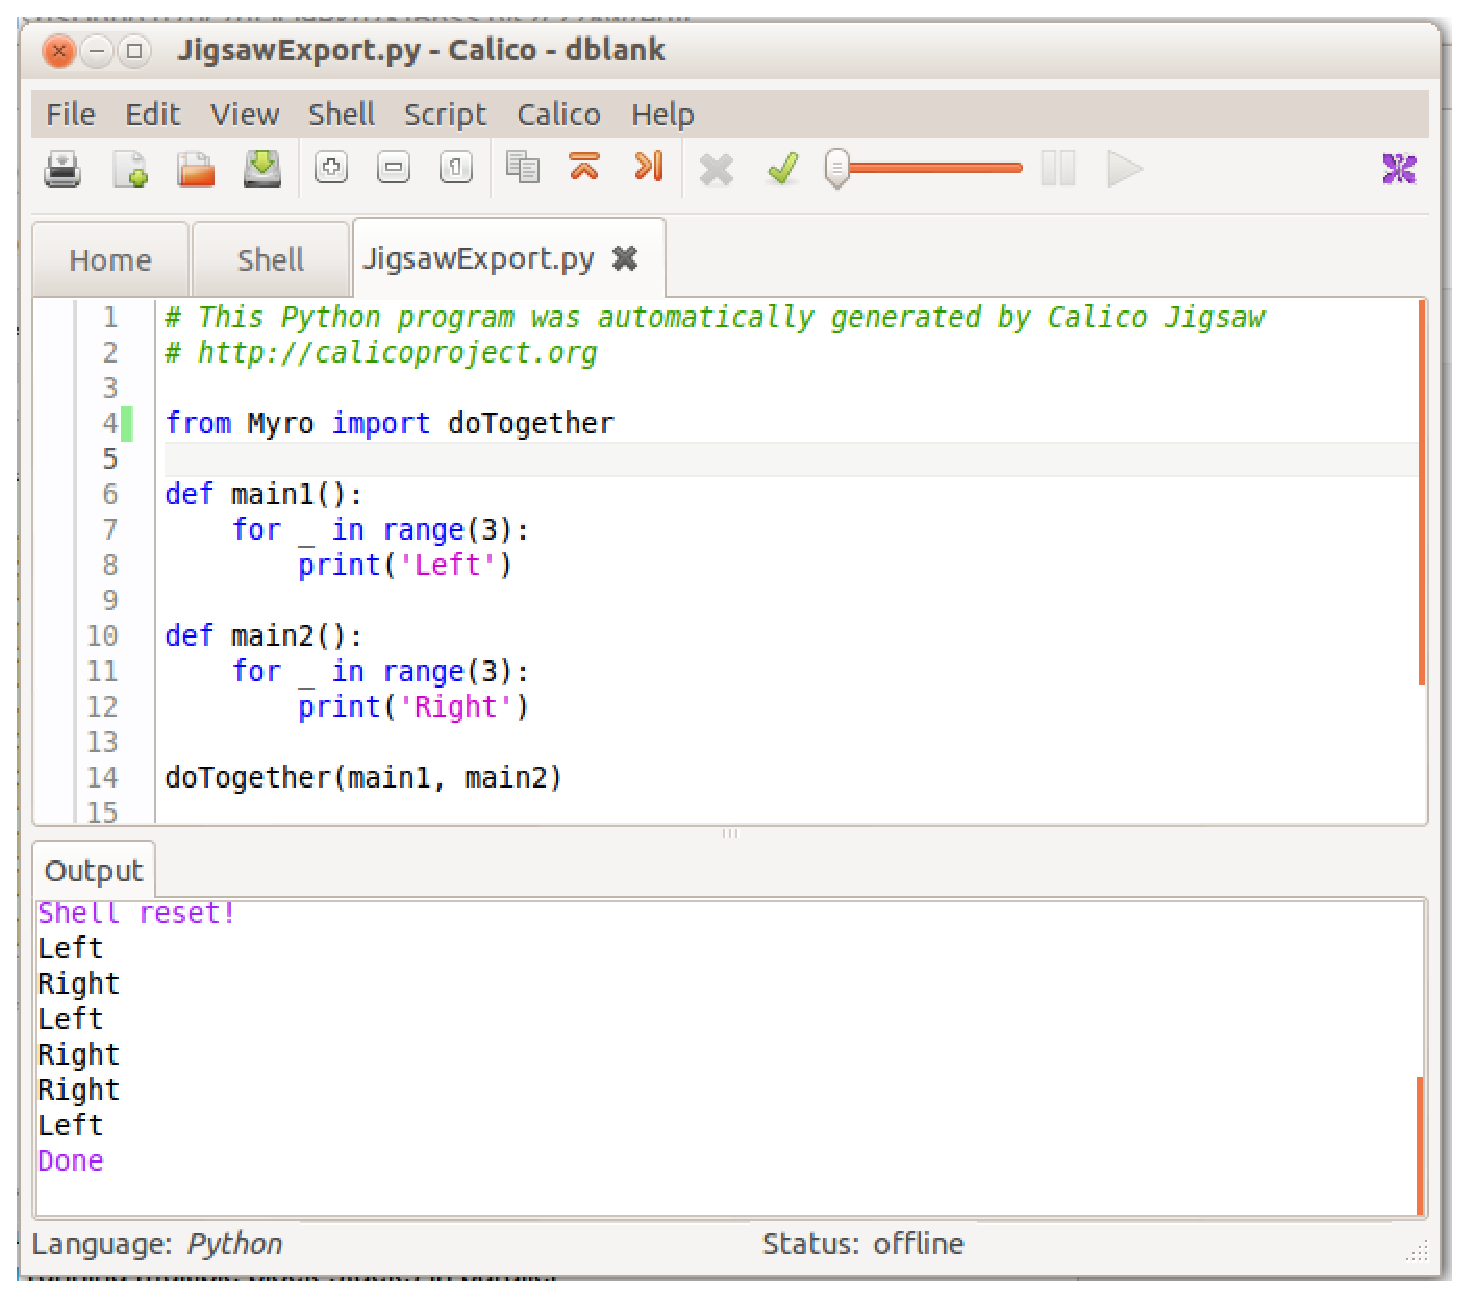
\includegraphics[width=75mm]{jigsaw4.eps} 
  \caption{The Jigsaw program from Figure~\ref{jigsaw3} exported
    Python. Note that the blocks have been converted to functions
    (main1, and main2) but the output is not guaranteed to run in
    lockstep as it does with Jigsaw's multitasking.}
  \label{jigsaw4}
\end{figure}

\subsection{Calico Python}

Based on IronPython. 

\subsection{Calico Ruby}

\subsection{Calico Scheme}

We wrote a properly tail-recursive implementation of Scheme from
scratch and integrated it into Calico.  Tail-recursion is an idiom that
students often discover on their own as a way of implementing
iteration (Blank and Kumar, 2010). Unfortunately, most of the
languages commonly used in introductory courses (for example, Java,
Python, and C++) do not handle tail-recursion correctly, which may
lead to crashes if a student’s program exceeds the language’s
recursion depth limit. This is seen by students as a bug in their
code, whereas it is really a limitation of the underlying language
implementation. Unlike other Scheme implementations for the MVM,
Calico Scheme does not rely on the underlying call stack of the
implementation language to manage function calls, nor does it require
functions to be compiled to Common Language Runtime (CLR)
bytecode. Consequently, tail calls are handled properly in Calico
Scheme, as required by the Scheme language specification (Sperber et
al., 2010), imposing no limit on the depth of the call stack (aside
from system memory limitations).

Scheme has two forms of a stack-trace when an exception is thrown,
depending on a user-set config. These are made to mimic those
stack-traces of Python.

\subsection{Experimental Languages}

To add a language to Calico, one need only define a single function
that returns a class instance. In fact, Calico comes with a
fill-in-the-blank wizard for creating new text-based languages. For
text-based languages, one need only provide the language's name, a
string for beginning line comments, and the the language's source code
file extension (such as ``.py'' for the Python language). Further
refinements can help make the language more useful for
programmers. Such refinements include providing language keyword
details for the IDE's color syntax highlighting, and, of course, the
language's parser and interpreter. Because Calico supports language
interoperations, new Calico languages can be written in existing
Calico languages. For example, Calico's Basic and Logo languages are
themselves written in Calico Python. As another example, Calico Java's
language definition is written in Python, but the Java interpreter is
written in Java (described in more detail below).

One might want to use the Calico infrastructure for testing out a new
language. For example, if you had an interpreter (written in any
Calico language, or converted to use the MVM or JVM) then you could
put a light wrapper around it, and simple use the Calico IDE to make
it easy to use. If you list the keywords, and a few other items, you
could also have color syntax highlighting. If you add hooks to your
language to import Calico modules, then your experimental language
would have access to all of the included libraries (described
below). Finally, if you add a method to provide line numbers, and
intercept breakpoints, then your language would also be a first-class
Calico language.

Because it is so easy to add a new language to Calico (given that such
a language might initially be a second-class language with little
connection to the rest of Calico) there are a few languages that have
been initiated.

\subsubsection{Calico Java}

Calico Java is an example of a second-class language in the ecosystem.

Java interpreter from DrJava written in Java. Java bytecode converted
to MVM bytecode. Thus, can parse and interpret Java in the MVM. Even
more interesting, the Calico modules can be used in the Java.

\subsubsection{Calico Basic, Logo}

Written in Calico Python. 

\subsection{Interoperations}

First class languages can call functions and use values
directly. Executing statements and expressions from another language.
Sharing values between languages.  Sharing code between languages.

Examples of interop.

\begin{verbatim}
scheme> (define pytuple 
          (calico.Evaluate "lambda *args: args" 
                           "python"))
Ok
scheme> (pytuple 1 2 3)
(1, 2, 3)
Ok
\end{verbatim}


\begin{verbatim}
scheme> (define pylist 
           (calico.Evaluate "lambda *args: list(args)" 
                            "python"))
Ok
scheme> (pylist 1 2 3)
[1, 2, 3]
Ok
\end{verbatim}

For example, in Python you can call a function written in Scheme.

\begin{enumerate}
\item First, write a regular Scheme function
\item Call the Scheme function in a CLR-compatible function wrapper
\item Make the wrapper available in the shared environment
\end{enumerate}

If one of the languages is not a first class Calico language, they can
still interoperate. For example, Java is not currently a first class
Calico language, but you can still execute statements, and evaluate
expressions from any language that has access to the calico
object. Here, Calico Python calls Java to create a variable with a
particular value:

\begin{verbatim}
python> calico.Execute("int x = 1;", "java")
True
Ok
python> py_x = calico.Evaluate("x", "java")
Ok
python> py_x
<java.lang.Integer object at 0x002B [1]>
python> py_x.intValue()
1
Ok
\end{verbatim}

The value of py\_x is actually value directly from the Java world: a
java.lang.Integer object. To convert it to a MVM value depends on the
specifics of the foreign system. In this case, py\_x.intValue().

\subsection{Current Limitations and Future Work}

Calico cannot currently use C-based libraries.
Limited exports from one language to another.
Move languages from second-class to first-class languages.

In addition, Kolling mentioned in his keynote address at SIGCSE this
year that he believes that we may be ready for a "structural editors"
rebirth. And this would be for experts. Paraphrasing, his idea is to
blend text editing with the idea of blocks (or "structures"). We can
tip our hat to the idea that "blocks" can be productive to experts
too.

\section{Calico Modules}

A Calico ``module'' is a library written in such a manner that it is
available to all of the Calico first-class languages. However, not
only is the functionality in the module available to these languages,
but the modules appear as if the are a native library to each
language. For example, in Calico Python one would write ``import
Processing'' to make the Calico Processing module (discussed below)
available to Python. One could then write ``Processing.window(400,
300)'' in Python to create a 400x300 pixel window. In Scheme, one
would write ``(using "Processing")'' to make the Calico Processing
module available to Scheme. One could then write ``(Processing.window
400 300)'' in Scheme to do the same thing. Finally, in Calico Jigsaw,
selecting ``Use a Module -> Processing'' from the menu would allow the
window-block to be dragged onto the Jigsaw workspace. Thus, the
Processing module is written and compiled once, becomes available to
all of the first-class Calico languages, and used as if it were
written as a native language. Likewise, if a new first-class language
is introduced into the Calico ecosystem, all of these modules can be
used by the new language.

To create a Calico module, a single file is written and compiled once
to a Dynamic Link Library (DLL). There are DLL files that are
Windows-specific; however, these DLLs are platform-neutral and can be
created on any operating system for use on any other operating
system. To remain platform-neutral these DLL's must be written such
that they do not take advantage of Windows-specific functionality, do
not rely on lower-level platform-specific C libraries (e.g., are
completely ``managed''), and use a subset of all possible
functionality. Currently, to be accessible to all Calico languages, we
currently restrict the module to only use static class methods in a
toplevel-defined class. However, this limit could be relaxed in a
future Calcio to allow more flexibility (constructors, nested classes,
etc). In general, any managed DLL could be fully utilized by a
properly flexible, dynamic, first-class languages, but might require
specific knowledge about the layout of the internal classes, methods,
and namespaces. Thus, we have specified a subset of all that is
possible for our own modules so that no additional knowledge or
discovery is needed.

\begin{verbatim}
public class ModuleName {
    public static int Plus(int a, int b) {
        return (a + b);
    }
}
\end{verbatim}

If the code in Figure was compiled and placed into the Calico/modules
folder, then it could be used in Python (as in the form ``import
ModuleName''), Scheme (as in the form ``(use "ModuleName")'' and in
Jigsaw and all of the other Calico languages, in their respective
forms. We now explore three modules that provided a variety of
functionality for Calico first-class languages.

\subsection{Processing}

Calico Processing is a module for developing digital works of art,
data visualizations, interactive applications and animations. It
offers Calico programmers the option to work with the familiar
Processing command set (see http://processing.org/reference). The
Calico Processing module attempts to be faithful to the Processing
command set, including function names, arguments, and usage. The
majority of the command set has been implemented, although some
differences exist.

The Processing language is a subset of Java with a wide variety of
commands included for creating visualization and animations. The
Calico Processing module brings the Processing command set to Calico
programming languages. This module does not make use of the Java
language syntax. Instead, native data types and control structures of
your chosen Calico language will determine how your application is
constructed.

We rely upon each of the native Calico languages for the following capabilities:

\begin{itemize}
\item Data structures
\item Program control (conditionals, iterations, etc.)
\item Files and file access
\item String functions
\item Objects and inheritance
\end{itemize}

Mouse and keyboard events are not handled by implementing predefined
functions. The Calico Processing module raises events, which are
handled by the native language event handling syntax. Events raised by
the module include onMousePressed, onMouseReleased, onMouseClicked,
onKeyPressed, and onKeyReleased.

Loops are implemented by handling a timer tick event named onLoop.

Certain predefined fields in Processing are implemented as functions.

\begin{itemize}
\item ''mouseX'' and ''mouseY'' are implemented in Calico Processing as the functions ''mouseX()'' and ''mouseY()''.
\item ''pmouseX'' and ''pmouseY'' are implemented as ''pmouseX()'' and ''pmouseY()''.
\item ''width'' and ''height'' are implemented as ''width()'' and ''height()''.
\item ''focused'' and ''frameCount'' are implemented as ''focused()'' and ''frameCount()''.
\item ''key'' and ''keyCode'' are implemented as ''key()'' and ''keyCode()''.
\end{itemize}

The result is a pixel-by-pixel faithful representation of the original
Processing primitives' output. However, combined with the Calico
dynamic languages, the Processing module provides functionality not
available within the original Processing environment. For example,
Calico allows the drag-and-drop creation of Processing art via Jigsaw,
line-by-line stepping through programs, and breakpoints by using any
of the Calico first-class languages.

\subsection{Myro}

Calico comes with a rich library for exploring robots, called
Myro. The Myro module allows students to control a real or simulated
robot, take pictures, do image processing, make the robot speak, go
through a maze, draw a picture, etc.

\subsection{Graphics}

This section describes Calico Graphics, a 2D graphics library for
creating art, games, and animations in any of the Calico languages.

\section{Conclusion}

%%\appendix
%%\section{Appendix Title}

%%This is the text of the appendix, if you need one.

\acks

Acknowledgments, if needed.

% We recommend abbrvnat bibliography style.

\bibliographystyle{abbrvnat}

% The bibliography should be embedded for final submission.

\begin{thebibliography}{}
\softraggedright

\bibitem[Smith et~al.(2009)Smith, Jones]{smith02}
P. Q. Smith, and X. Y. Jones. ...reference text...

\bibitem[Da Vinci (2008)]{davinci}
%% Details on Da Vinci Machine for the JVM
%% http://openjdk.java.net/projects/mlvm/pdf/LangNet20080128.pdf

\bibitem[Rose (2012)]{jrose12}
%% Details on upcoming dynamic language support for Java
%% http://cr.openjdk.java.net/~jrose/pres/201204-LangNext.pdf

\bibitem[]{squeak}
%% Lists many via VMs, including Squeak
%% http://en.wikipedia.org/wiki/Comparison_of_application_virtual_machines

\end{thebibliography}

\end{document}

